%\title{Project Report}
%
%%% Preamble
\documentclass[paper=a4, fontsize=11pt]{scrartcl}
\usepackage[T1]{fontenc}
\usepackage{fourier}

\usepackage[english]{babel}															% English language/hyphenation
\usepackage[protrusion=true,expansion=true]{microtype}	
\usepackage{amsmath,amsfonts,amsthm} % Math packages
\usepackage[pdftex]{graphicx}	
\usepackage{url}
\usepackage{listings}


\usepackage[final]{pdfpages}
\usepackage[section]{placeins}

%%% Custom sectioning
\usepackage{sectsty}
\allsectionsfont{\centering \normalfont\scshape}


%%% Custom headers/footers (fancyhdr package)
\usepackage{fancyhdr}
\pagestyle{fancyplain}
\fancyhead{}											% No page header
\fancyfoot[L]{}											% Empty 
\fancyfoot[C]{}											% Empty
\fancyfoot[R]{\thepage}									% Pagenumbering
\renewcommand{\headrulewidth}{0pt}			% Remove header underlines
\renewcommand{\footrulewidth}{0pt}				% Remove footer underlines
\setlength{\headheight}{13.6pt}


%%% Equation and float numbering
\numberwithin{equation}{section}		% Equationnumbering: section.eq#
\numberwithin{figure}{section}			% Figurenumbering: section.fig#
\numberwithin{table}{section}				% Tablenumbering: section.tab#


%%% Maketitle metadata
\newcommand{\horrule}[1]{\rule{\linewidth}{#1}} 	% Horizontal rule

\title{
		%\vspace{-1in} 	
		\usefont{OT1}{bch}{b}{n}
		\normalfont \normalsize \textsc{University of Michigan} \\ [25pt]
		\horrule{0.5pt} \\[0.4cm]
		\huge AERO 584, Homework  5 \\
		\horrule{2pt} \\[0.5cm]
}
\author{
		\normalfont 								\normalsize
         Huckleberry Febbo\\[-3pt]		\normalsize
        \today
}
\date{}

%%%%%%%%%%%%%%%%%%%%%%%%%%%%%%%%%%%%%%%%%%%%%%%%%%%%%%%%%%%%%%%%%%%%%
%%%%%%%%%%%%%%%%%%%%%%%%%%%%%%%%PACKAGES%%%%%%%%%%%%%%%%%%%%%%%%%%%%%%%%

% *** MATH ***
\usepackage{amsmath}
\usepackage{cases}
\usepackage{mathrsfs}
\usepackage{amssymb}
\DeclareMathAlphabet\mathbfcal{OMS}{cmsy}{b}{n}


% *** GRAPHICS ***
\usepackage[]{graphicx}
\usepackage{epstopdf}
\usepackage{svg}
\setsvg{inkscape=inkscape -z -D,svgpath=figs/}

\usepackage{lineno,hyperref}
\modulolinenumbers[5]


\bibliographystyle{elsarticle-num}
%%%%%%%%%%%%%%%%%%%%%%%

\begin{document}
\maketitle

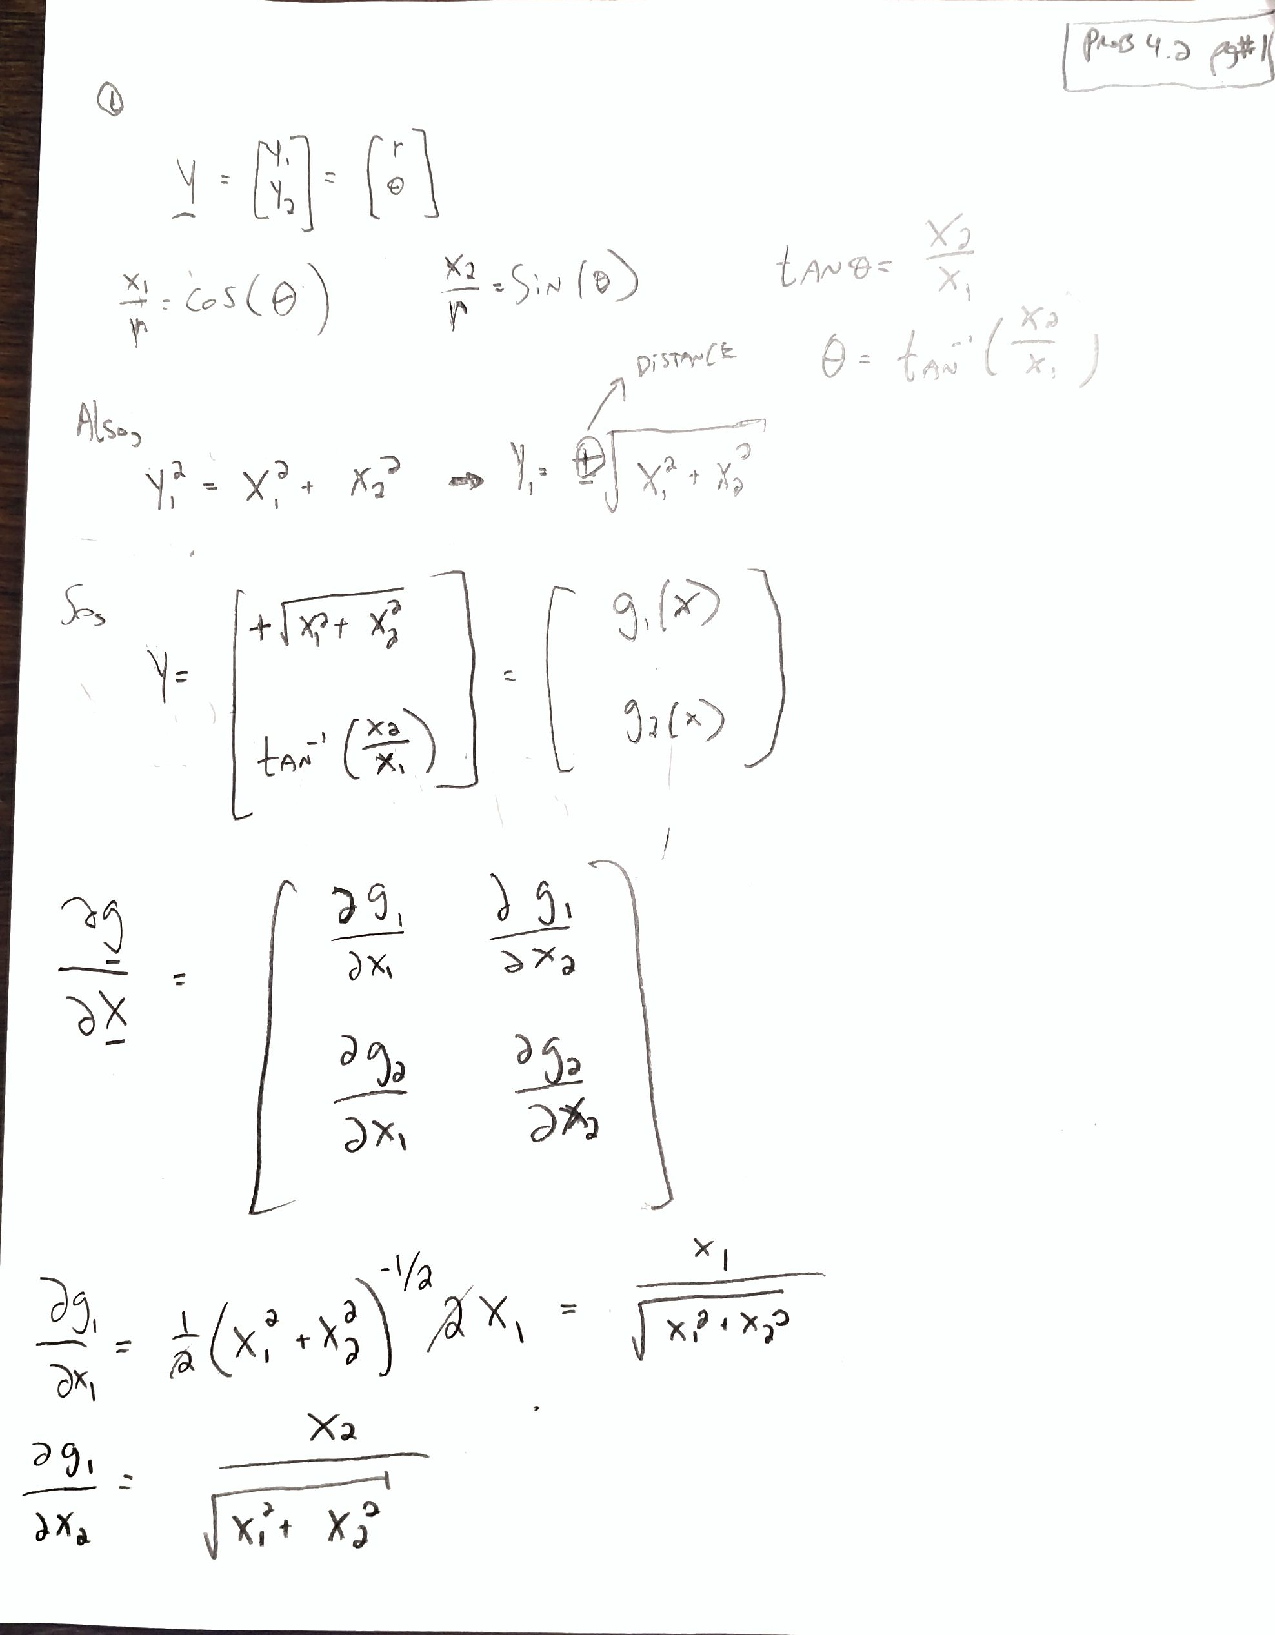
\includepdf[pages=-]{probs.pdf}

\section*{Problem 4.10, continued}

Similar to the result that is seen in Problem 4.15, Part 3, even though the system is not observable, but it is detectable; meaning that even though the eigenvalues of the matrix $A+GC$ cannot all be placed using $G$, the ones that cannot be palaced are negative, so they the estimates will converge asymtotically to zero. For this case, because $A_11$ is asmptotically stable and the pair $(A_{22},C_2)$ is completely observable the gain, $g_2$ can be designed so that $A_{22} + g_2C_2$ is stable and thus the states can be reconstructed.

%\textbf{LaTeX moved my figures, but they are all there }
\section*{Problem 4.15, Part 1}



Given the pulse input shown in the bottom of Fig. \ref{fig:f1}, the reponses for both the actual system and the symptotic observer can alse be seen in Fig. \ref{fig:f1}. 

\begin{figure}[!htb]
	\centering
    \includesvg[width=0.9\textwidth]{p1_4_15}
	\caption{Actual system response compared to asmptotic observer shown for a pulse input. $g1= -10$\label{fig:f1}}
\end{figure}
It can be seen that while the heading angle is accurately reconstructed, both the roll angle and the roll angle rate are not. For the results in Fig. \ref{fig:f2}, $g1$ is decreased by an order of magnitude and it can be seen that all of the states are not accurately reconstructed.
\begin{figure}[ht]
	\centering
    \includesvg[width=0.7\textwidth]{p1_4_15_2}
	\caption{Actual system response compared to asmptotic observer shown for a pulse input, $g1 = -100$ \label{fig:f2}}
\end{figure}



\section*{Problem 4.15, Part 2}

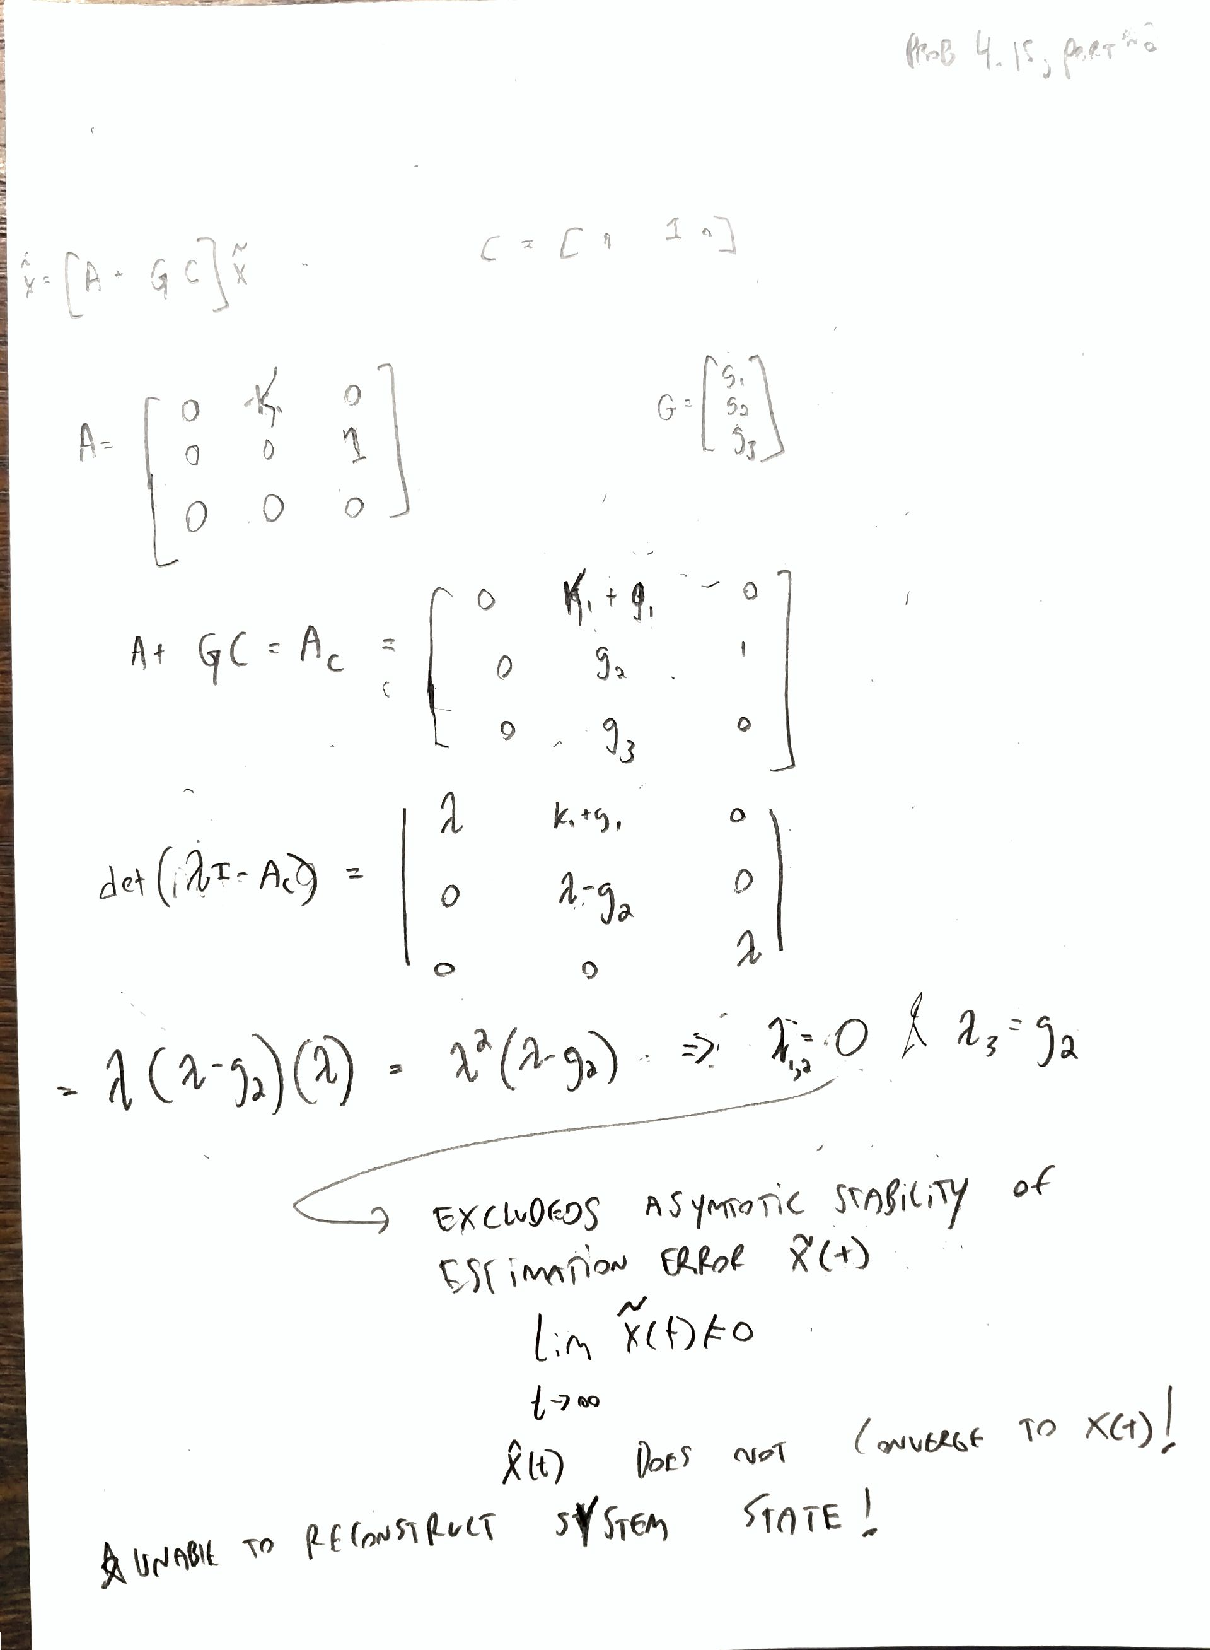
\includepdf[pages=-]{p1_2.pdf}

Next in Fig. \ref{fig:f3} and Fig. \ref{fig:f4} (longer simulation time), it can be seen that the roll angle is able to be reconstructed, but the observer does a poor job with the other two states.

\begin{figure}[!htb]
	\centering
    \includesvg[width=0.5\textwidth]{p2_4_15}
	\caption{System response with asymtotic observer compared to actual system response; for a step input. \label{fig:f3}}
\end{figure}

\begin{figure}[!]
	\centering
    \includesvg[width=0.5\textwidth]{p2_4_15_2}
	\caption{System response with asymtotic observer compared to actual system response; for a step input. \label{fig:f4}}
\end{figure}

\section*{Problem 4.15, Part 3}
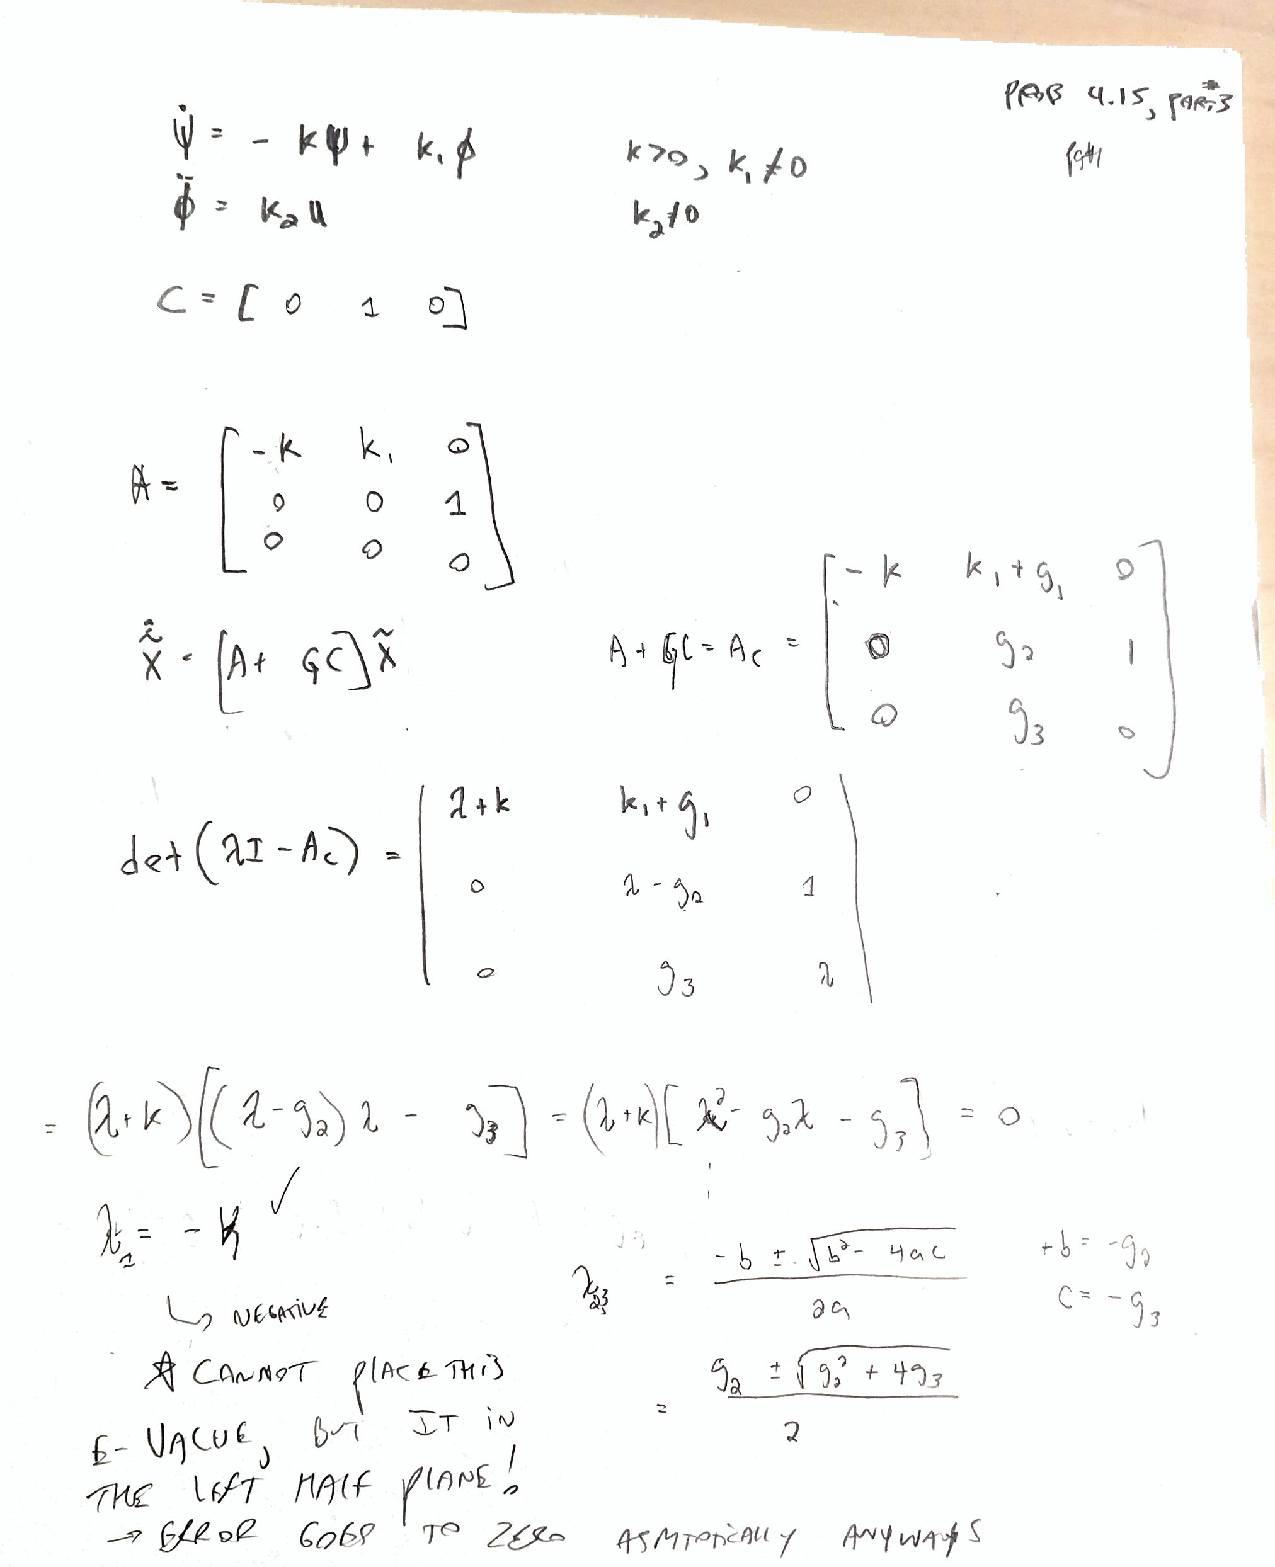
\includepdf[pages=-]{prob3.pdf}

\begin{figure}[!htb]
	\centering
    \includesvg[width=0.9\textwidth]{p3_4_15}
	\caption{System response with asymtotic observer compared to actual system response; for a step input. \label{fig:f5}}
\end{figure}

\section*{Problem 4.16, Part 1}

\textbf{Linear Gauss-Markov Model} \\
The standard model is:
\begin{align}
\dot{x}(t)&=A(t)x(t)+B(t)u(t)+w(t), t \geq t_0\\
y(t)&=C(t)x(t)+v(t)
\end{align}

For our time invariant case:
\begin{align}
\dot{x}(t)&=Ax(t)+Bu(t)+w(t), t \geq t_0\\
y(t)&=Cx(t)+v(t)
\end{align}

With,
\begin{align*}
A=
\begin{bmatrix}
0& -k_1 &0\\
0 &0& 1\\
0 &0& 0\\
\end{bmatrix}
\end{align*}
\begin{align*}
C=
\begin{bmatrix}
1& 0 &0\\
\end{bmatrix}
\end{align*}
\begin{align*}
w(t)=
\begin{bmatrix}
0\\
0\\
w_{\dot{\phi}}(t)\\
\end{bmatrix}
\end{align*}
\begin{align*}
v(t)=
\begin{bmatrix}
v_{\psi}(t)\\
0\\
0\\
\end{bmatrix}
\end{align*}

also, \\
$$v_{\psi}(t) = N(0,\sigma_v^2)$$ 

$$w_{\dot{\phi}}(t) = N(0,\sigma_w^2)$$

\begin{align*}
R_w=
\begin{bmatrix}
0 & 0 & 0\\
0 & 0 & 0\\
0 & 0 & \sigma_w^2 \\
\end{bmatrix}
\end{align*}
\begin{align*}
R_v=\sigma_v^2
\end{align*}
\begin{align*}
A^T=
\begin{bmatrix}
0 & 0 & 0\\
-k_1 & 0 & 0\\
0 & 1 & 0 \\
\end{bmatrix}
\end{align*}
\begin{align*}
P=
\begin{bmatrix}
p_1 & p_2 & p_3\\
p_2 & p_5 & p_6\\
p_3 & p_6 & p_9 \\
\end{bmatrix}
\end{align*}

\textbf{Steady-State Covariance Matrix}\\

\textbf{Differential Riccati Equation}
the optimal covariance matrix satisfies:
\begin{align*}
\dot{P}(t)&=A(t)P(t)+P(t)A^T(t)-P(t)C(t)^TR^{-1}_{v}(t)C(t)P+R_w(t)\\
P(t_0)&=P_0
\end{align*}
\textbf{Algebraic Riccati Equation}
The steady-state covariance matrix, $P$ for our time-invariant problem is the solution to:
\begin{align*}
AP+PA^T-PC^TR^{-1}_{v}CP+R_w=0
\end{align*}
\begin{align*}
\begin{bmatrix}
0& -k_1 &0\\
0 &0& 1\\
0 &0& 0\\
\end{bmatrix}
\begin{bmatrix}
p_1 & p_2 & p_3\\
p_2 & p_5 & p_6\\
p_3 & p_6 & p_9 \\
\end{bmatrix}+
\begin{bmatrix}
p_1 & p_2 & p_3\\
p_2 & p_5 & p_6\\
p_3 & p_6 & p_9 \\
\end{bmatrix}
\begin{bmatrix}
0 & 0 & 0\\
-k_1 & 0 & 0\\
0 & 1 & 0 \\
\end{bmatrix} \dots
\end{align*}
\begin{align*}
-
\begin{bmatrix}
p_1 & p_2 & p_3\\
p_2 & p_5 & p_6\\
p_3 & p_6 & p_9 \\
\end{bmatrix}
\begin{bmatrix}
1\\
0\\
0\\
\end{bmatrix}\frac{1}{\sigma_v^2}
\begin{bmatrix}
1&0&0\\
\end{bmatrix}
\begin{bmatrix}
p_1 & p_2 & p_3\\
p_2 & p_5 & p_6\\
p_3 & p_6 & p_9 \\
\end{bmatrix}
+
\begin{bmatrix}
0 & 0 & 0\\
0 & 0 & 0\\
0 & 0 & \sigma_w^2 \\
\end{bmatrix}=0
\end{align*}
\begin{align*}
\begin{bmatrix}
-k_1p_2&-k_1p_5&-k_1p_6\\
p_3&p_6&p_9\\
0&0&0
\end{bmatrix}+
\begin{bmatrix}
-p_2k_1&p_3&0\\
-p_5k_1&p_6&0\\
-k_1p_6&p_9&\sigma_w^2
\end{bmatrix}-\frac{1}{\sigma_v^2}
\begin{bmatrix}
p_1^2&p_1p_2&p_1p_3\\
p_1p_2&p_2^2&p_2p_3\\
p_1p_3&p_2p_3&p_3^2
\end{bmatrix}=0
\end{align*}
\begin{align*}
\begin{bmatrix}
-k_1p_2-p_2k_1-\frac{1}{\sigma_v^2}p_1^2&-k_1p_5+p_3-\frac{1}{\sigma_v^2}p_1p_2&-k_1p_6-\frac{1}{\sigma_v^2}p_1p_3\\
p_3+-p_5k_1-\frac{1}{\sigma_v^2}p_1p_2&2p_6-\frac{1}{\sigma_v^2}p_2^2&p_9-\frac{1}{\sigma_v^2}p_2p_3\\
-k_1p_6-\frac{1}{\sigma_v^2}p_1p_3&p_9-\frac{1}{\sigma_v^2}p_2p_3&\sigma_w^2-\frac{1}{\sigma_v^2}p_3^2
\end{bmatrix}=0
\end{align*}
Then using julia,
\begin{tiny}
\begin{lstlisting}
using SymPy
@syms p1 p2 p3 p5 p6 p9 k1 sigma_w sigma_v
k1 = symbols("k1",nonzero=true, real=true)
p1,p2,p3,p4,p5,p6,p9,sigma_w,sigma_v = symbols("p1,p2,p3,p4,p5,p6,p9,sigma_w,sigma_v",real=true)
exs = [-k1*p2-p2*k1-1/sigma_v^2*p1^2, -k1*p5+p3-1/sigma_v^2*p1*p2,-k1*p6-1/sigma_v^2*p1*p3,p9-1/sigma_v^2*p2*p3,2*p6-1/sigma_v^2*p2^2,sigma_w^2-1/sigma_v^2*p3^2]
d = solve(exs,[p1,p2,p3,p4,p5,p6,p9])
\end{lstlisting}
\end{tiny}

which gives,
\begin{lstlisting}
 Dict(p2=>0,p5=>sigma_v*sigma_w/k1,p9=>0,p6=>0,p3=>sigma_v*sigma_w,p1=>0)                                                                                                                                                                                                                                                                                                                                                                                                                                                                                                                                                                         
\end{lstlisting}
So,
\begin{align*}
P=
\begin{bmatrix}
0 & 0 & \sigma_w \sigma_v\\
0 & \frac{\sigma_v \sigma_w}{k_1} & 0\\
\sigma_w \sigma_v & 0 & 0 \\
\end{bmatrix}
\end{align*}
\textbf{Optimal Kalman Gain}\\
$$G=-PC^TR^{-1}_{v}$$
\begin{align*}
-\begin{bmatrix}
0 & 0 & \sigma_w \sigma_v\\
0 & \frac{\sigma_v \sigma_w}{k_1} & 0\\
\sigma_w \sigma_v & 0 & 0 \\
\end{bmatrix}
\begin{bmatrix}
1\\
0\\
0\\
\end{bmatrix}
\frac{1}{\sigma_v^2}=-
\begin{bmatrix}
0\\
0\\
\frac{\sigma_w}{\sigma_v}
\end{bmatrix}
\end{align*}
\section*{Problem 4.16, Part 2}
Yes. The stability analysis performed helps identify what the gains need to be for a stable system, this can help us to draw conculsions about what vaules the standard deviations should be for good performance.
\section*{Problem 4.16, Part 3}

In Fig. \ref{fig:f41} the response can be seen for $\frac{\sigma_w}{\sigma_v} =  .001 << 1$ and in Fig. \ref{fig:f40} the response can be seen for $\frac{\sigma_w}{\sigma_v} =  100 >> 1$. Notice that in the first case, the response is stable and in the second case, the response is unstable. 
\begin{figure}
	\centering
    \includesvg[width=0.8\textwidth]{p1_4_16_2}
	\caption{System response with Kalman-filter compared to actual system response; for a pulse input. $\frac{\sigma_w}{\sigma_v} =  .001 << 1$ \label{fig:f41}}
\end{figure}

\begin{figure}
	\centering
    \includesvg[width=0.8\textwidth]{p1_4_16}
	\caption{System response with Kalman-filter compared to actual system response; for a pulse input. $\frac{\sigma_w}{\sigma_v} =  100 >> 1$ \label{fig:f40}}
\end{figure}
\end{document}
